\chapter{التنظيم الوظيفي عند النبات الزهري}\label{ch:b1:flowering-plant-organization}

بلوطة عمرها قرنان تقف في المتر المربع نفسه من الأرض الذي أنبتت فيه.
لم تأكل قط، ولم تتحرك قط، ولم تضبط حرارتها قط؛ ومع ذلك بنت أربعين
طنًا من \omterm{def:b1:flowering-plant-organization:tissues}{الخشب}، وهي تنشر كل صيف خمسمئة متر مربع من الورق في الهواء،
وسطحًا أكبر من \omterm{def:b1:flowering-plant-organization:organs}{الجذر} في التربة. النبات الزهري هو الجواب الآخر عن
مشكلة \cref{ch:b1:organism-environment}: ذاتي تغذٍ ثابت في مكانه
يلاقي محيطه لا بإدخال تبادلاته إلى داخله بل بإنماء سطوح تبادله إلى
الخارج، بلا حد، حيثما كان الضوء والماء. يصف هذا الفصل كيف يُنظَّم
جسم كهذا --- أعضاؤه، وأنسجته، والسطوح التي ينشرها، والنمو الذي
يبنيها.

\begin{omfigure}
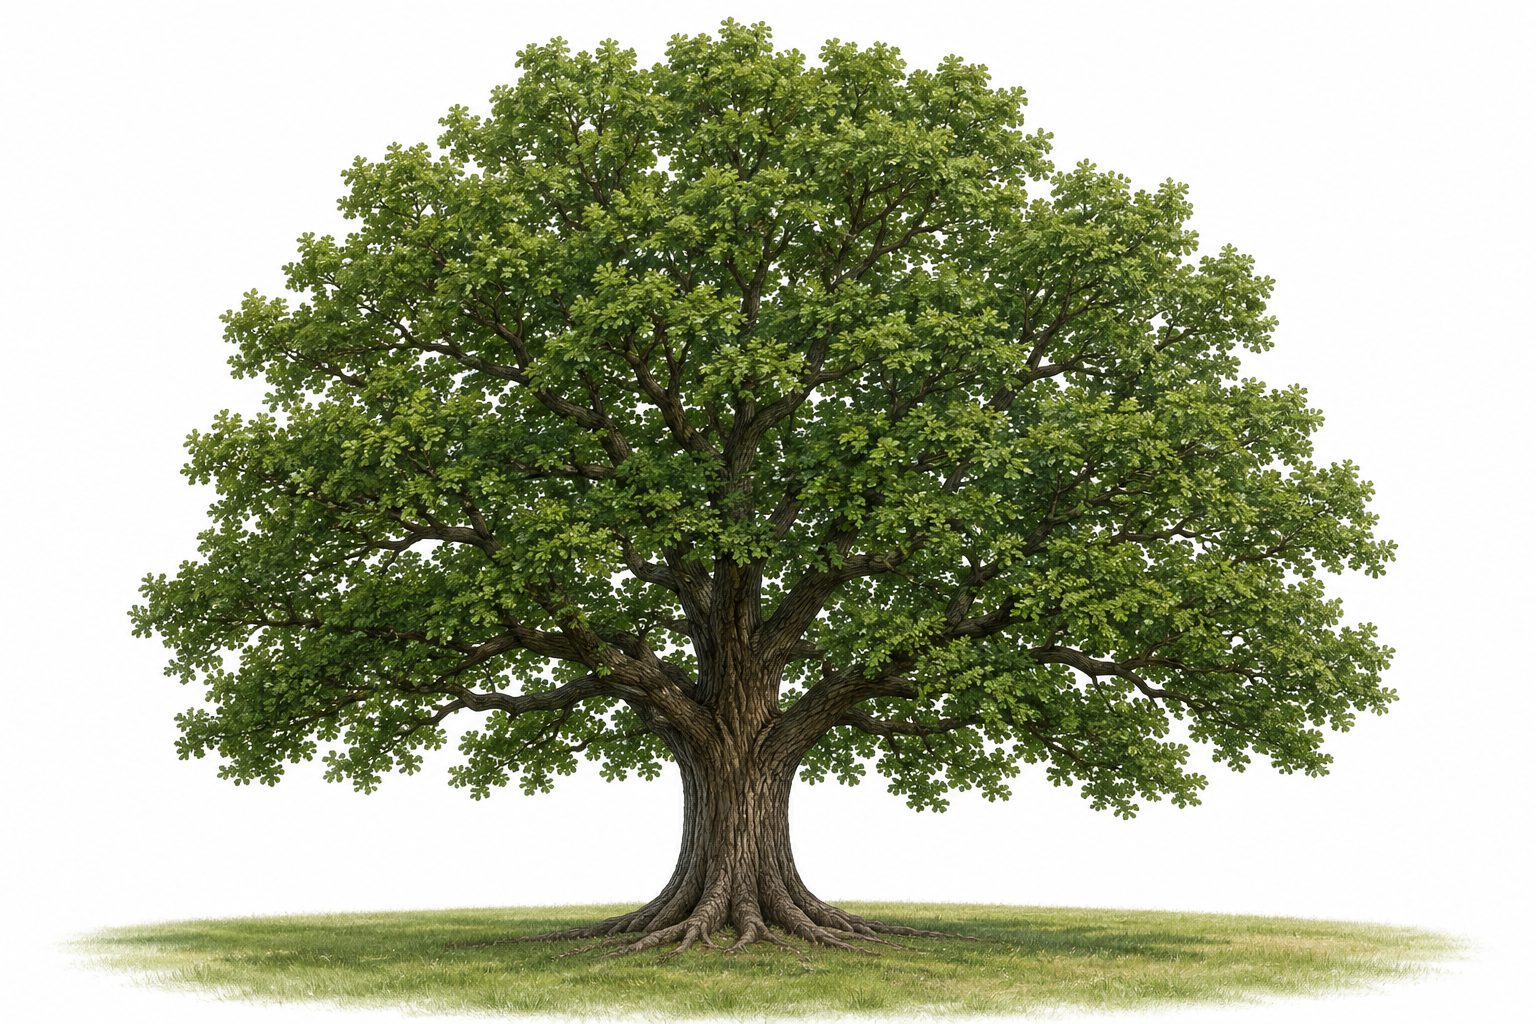
\includegraphics[width=0.62\linewidth]{images/book3/ai/b3-03-oak-tree.png}

{\small بلوطة منفردة في الصيف. تاجها صف من \omterm{def:b1:flowering-plant-organization:organs}{الأوراق} منشورة لاعتراض
الضوء؛ ومجموعها الجذري تحت العشب واسع سعة التاج وسطحه أكبر منه بمرات
عدة.}
\end{omfigure}

\section{الجسم الخضري}

\begin{definition}[الجذر والساق والورقة]\label{def:b1:flowering-plant-organization:organs}
يتكون الجسم الخضري للنبات الزهري من ثلاثة أنواع من \omterm{def:b1:mammal-organization:organ}{الأعضاء}.
\emph{الجذر}\index{جذر} يثبت النبات ويمتص الماء والشوارد المعدنية من
التربة؛ وهو ينمو من قمته، ويتفرع، ويحمل \emph{أشعارًا
جذرية}\index{شعرة جذرية} خلف القمة مباشرة. و\emph{الساق}\index{ساق}
يحمل الأوراق نحو الضوء وينقل بين الجذور والأوراق؛ وهو مبني من وحدات
متكررة، كل منها \emph{عقدة}\index{عقدة} تحمل ورقة وبرعمًا إبطيًا،
و\emph{سلامية}\index{سلامية} بين عقدتين. و\emph{الورقة}\index{ورقة}
هي \omterm{def:b1:mammal-organization:organ}{عضو} التركيب الضوئي: نصل مسطح كبير السطح صغير السماكة، يحمله عنق.
والجذور تكوّن المجموع الجذري؛ والسيقان والأوراق تكوّن المجموع الخضري
الهوائي.
\end{definition}

\begin{proposition}[جسم وحدوي مفتوح]\label{prop:b1:flowering-plant-organization:modular}
جسم النبات \emph{وحدوي}\index{النمو الوحدوي}: فالمجموع الهوائي
سلسلة من وحدات متماثلة (\omterm{def:b1:flowering-plant-organization:organs}{عقدة}، \omterm{def:b1:flowering-plant-organization:organs}{وورقة}، وبرعم، \omterm{def:b1:flowering-plant-organization:organs}{وسلامية}) يضيفها برعم
قمي واحدة إثر أخرى، ويستطيع كل برعم إبطي أن يبدأ سلسلة جديدة. والنمو
\emph{غير محدود}\index{النمو غير المحدود}: فلا قياس بالغ، والنبات
يظل يضيف الوحدات، ومن ثم السطح، ما دام حيًا. وعدد الوحدات ومواضعها
يتوقفان على الموقع --- الضوء، والماء، والأذى --- فيتخذ النوع الواحد
أشكالًا مختلفة في أمكنة مختلفة. أما جسم الثديي فمغلق على العكس من
ذلك: أعضاؤه محددة العدد وهو يكف عن النمو عند قياس معين.
\end{proposition}

\begin{omfigure}
\begin{tikzpicture}[font=\small, >=Stealth, line cap=round]
  % stem axis
  \draw[very thick, omExo!70!black] (0,0) -- (0,6.2);
  \node[circle, fill=omExo!70!black, inner sep=2.2pt] at (0,6.2) {};
  \node[right, font=\footnotesize, align=left] at (0.25,6.35) {البرعم القمي: يضيف\\ وحدات جديدة فوق};
  % nodes with leaves and axillary buds
  \foreach \y/\side in {1.2/1, 2.6/-1, 4.0/1, 5.2/-1} {
    \fill[omExo!70!black] (0,\y) circle (2pt);
    \draw[thick, omExo!70!black] (0,\y) -- (\side*0.6,\y+0.25);
    \draw[thick, omExo, fill=omExo!30] (\side*0.6,\y+0.25) .. controls (\side*1.4,\y+0.6) and (\side*2.2,\y+0.15) .. (\side*2.0,\y-0.1) .. controls (\side*1.4,\y-0.25) and (\side*0.9,\y-0.05) .. (\side*0.6,\y+0.25);
    \fill[omProp] (\side*0.18,\y+0.28) circle (2pt);
  }
  % module bracket
  \draw[thick, gray] (-2.4,1.2) -- (-2.6,1.2) -- (-2.6,2.6) -- (-2.4,2.6);
  \node[left, font=\footnotesize, align=right, gray] at (-2.65,1.9) {وحدة واحدة:\\ سلامية، عقدة،\\ ورقة، برعم إبطي};
  \node[right, font=\footnotesize] at (2.2,4.1) {ورقة};
  \node[right, font=\footnotesize, omProp] at (0.25,2.95) {برعم إبطي};
  \node[left, font=\footnotesize] at (-0.3,3.3) {سلامية};
  \node[left, font=\footnotesize] at (-0.3,3.98) {عقدة};
  % roots
  \draw[very thick, omDef!70!black] (0,0) -- (0,-1.6);
  \draw[thick, omDef!70!black] (0,-0.5) -- (-1.0,-1.3) (0,-0.9) -- (0.9,-1.5) (0,-1.2) -- (-0.5,-2.0);
  \foreach \x in {-0.12,-0.06,0.06,0.12} \draw[omDef!70!black] (\x,-1.55) -- (\x*3,-1.9);
  \node[right, font=\footnotesize, align=left] at (0.5,-0.75) {المجموع الجذري: ينمو من\\ القمم، والأشعار الجذرية خلفها};
  \draw[dashed, gray] (-3.0,0) -- (3.2,0);
  \node[font=\footnotesize, gray, anchor=south east] at (3.2,0.02) {سطح التربة};
\end{tikzpicture}

{\small المجموع الهوائي كومة من الوحدات. كل عقدة تحمل \omterm{def:b1:flowering-plant-organization:organs}{ورقة} وبرعمًا
إبطيًا؛ والبرعم القمي يضيف وحدات فوق، وأي برعم إبطي يستطيع أن يبدأ
فرعًا. والمجموع الجذري ينمو من قممه.}
\end{omfigure}

\section{أنسجة الجسم الأولي}

\begin{definition}[النسيج الجلدي والأساسي والوعائي]\label{def:b1:flowering-plant-organization:tissues}
كل \omterm{def:b1:mammal-organization:organ}{عضو} من \omterm{def:b1:mammal-organization:organ}{أعضاء} النبات مبني من ثلاث جمل نسيجية. \emph{النسيج
الجلدي}\index{النسيج الجلدي} هو \emph{البشرة}\index{بشرة}، وهي طبقة
خلوية وحيدة تغطي \omterm{def:b1:mammal-organization:organ}{العضو}، مغلفة في الهواء \emph{بأديمة}\index{أديمة}
شمعية ومثقوبة \emph{بثغور}\index{ثغر}، وممتدة في \omterm{def:b1:flowering-plant-organization:organs}{الجذر} بأشعار
جذرية. و\emph{النسيج الأساسي}\index{النسيج الأساسي} يملأ \omterm{def:b1:mammal-organization:organ}{العضو}:
\emph{البرنشيم}\index{برنشيم} (خلايا حية رقيقة الجدر للتركيب الضوئي
والادخار)، و\emph{الكولنشيم}\index{كولنشيم} (خلايا حية جدرها مثخنة
تثخينًا غير منتظم، وهو الدعامة المرنة للسيقان الفتية)،
و\emph{السكلرنشيم}\index{سكلرنشيم} (خلايا ذات جدر متخشبة سميكة،
ميتة عند النضج، وهي الدعامة الصلبة: الألياف والخلايا الحجرية).
و\emph{النسيج الوعائي}\index{النسيج الوعائي} ينقل:
\emph{الخشب}\index{خشب} يحمل الماء والأملاح صعودًا في
\emph{القصيبات}\index{قصيبة} و\emph{الأوعية}\index{وعاء} الجوفاء
المتخشبة الميتة (\cref{ch:b1:plant-transport})؛
و\emph{اللحاء}\index{لحاء} يحمل السكريات في \emph{أنابيب
غربالية}\index{أنبوب غربالي} حية تبقيها حية خلاياها المرافقة.
\end{definition}

\begin{omfigure}
\begin{tikzpicture}
  \node[anchor=south west, inner sep=0] (img) at (0,0)
    {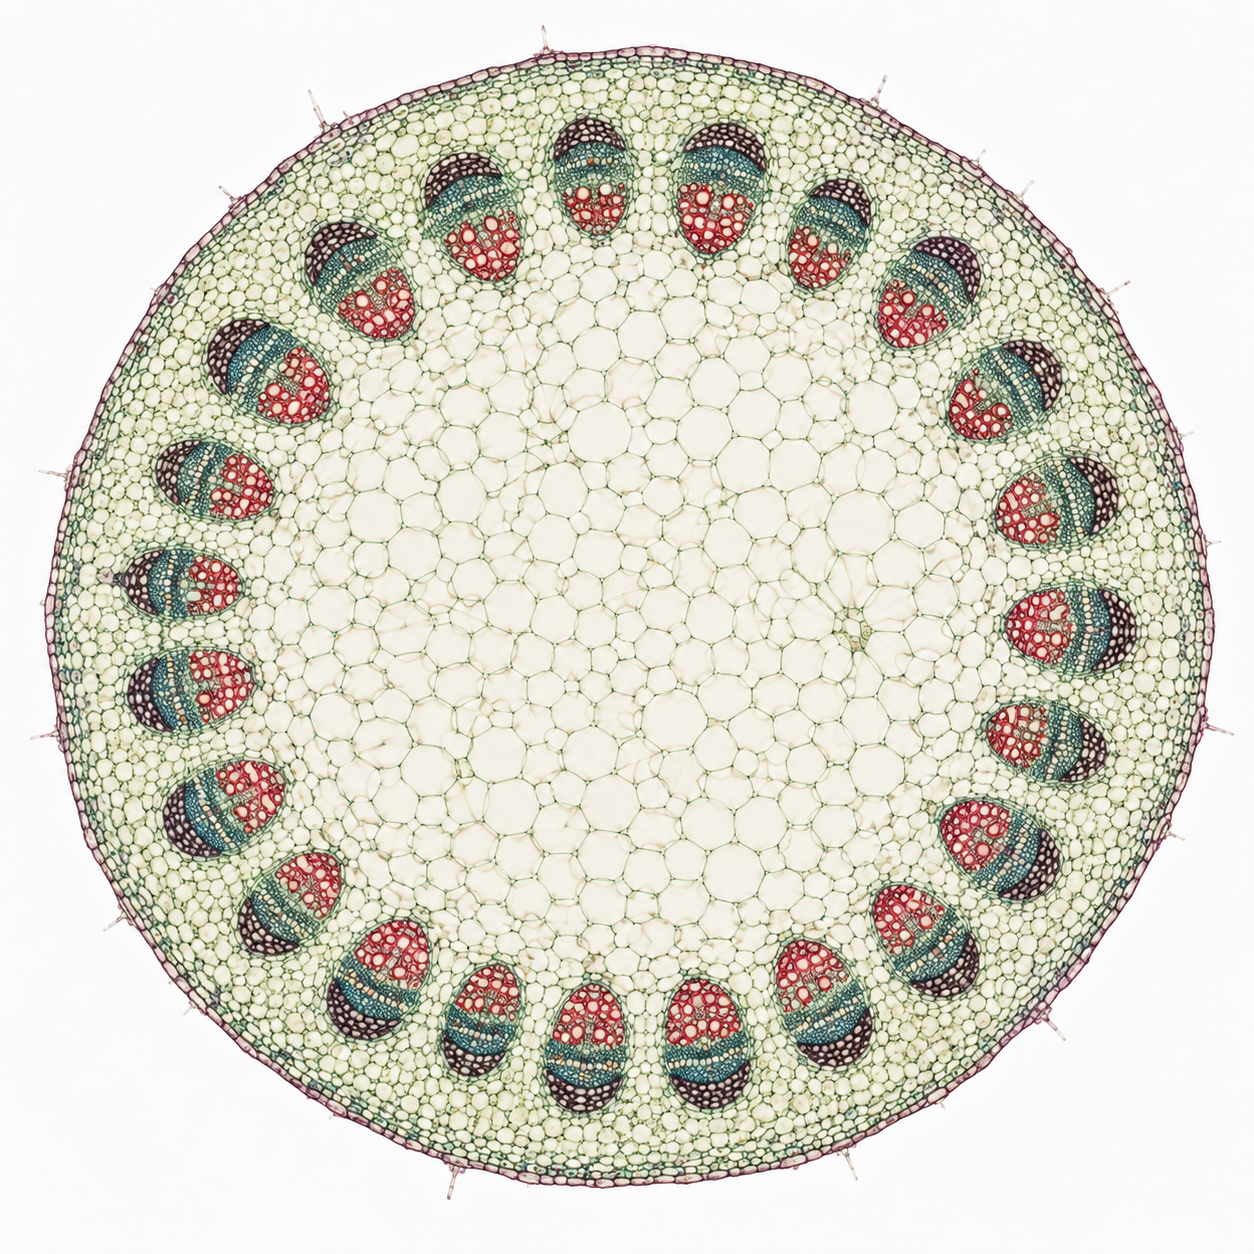
\includegraphics[width=0.5\linewidth]{images/book3/ai/fig-dicot-stem-cross.png}};
  \begin{scope}[x={(img.south east)}, y={(img.north west)},
      every node/.style={font=\small}]
    \draw[omDef, thick] (0.50,0.895) -- (0.50,1.06) node[above] {قلنسوة سكلرنشيم فوق حزمة};
    \draw[omDef, thick] (0.87,0.50) -- (1.03,0.60) node[right] {لحاء (إلى الخارج)};
    \draw[omDef, thick] (0.81,0.50) -- (1.03,0.42) node[right] {خشب (إلى الداخل)};
    \draw[omDef, thick] (0.50,0.50) -- (-0.03,0.50) node[left] {لب};
    \draw[omDef, thick] (0.085,0.56) -- (-0.03,0.66) node[left] {قشرة};
    \draw[omDef, thick] (0.06,0.40) -- (-0.03,0.32) node[left] {بشرة};
  \end{scope}
\end{tikzpicture}

{\small مقطع عرضي في ساق فتي ثنائي الفلقة. الحزم الوعائية تكوّن
حلقة: في كل منها يواجه \omterm{def:b1:flowering-plant-organization:tissues}{الخشب} (المصبوغ بالأحمر، المتخشب) المركز
ويواجه \omterm{def:b1:flowering-plant-organization:tissues}{اللحاء} الخارج، تحت قلنسوة من الألياف. وداخل الحلقة اللب،
وخارجها القشرة والبشرة.}
\end{omfigure}

\begin{omfigure}
\begin{tikzpicture}
  \node[anchor=south west, inner sep=0] (img) at (0,0)
    {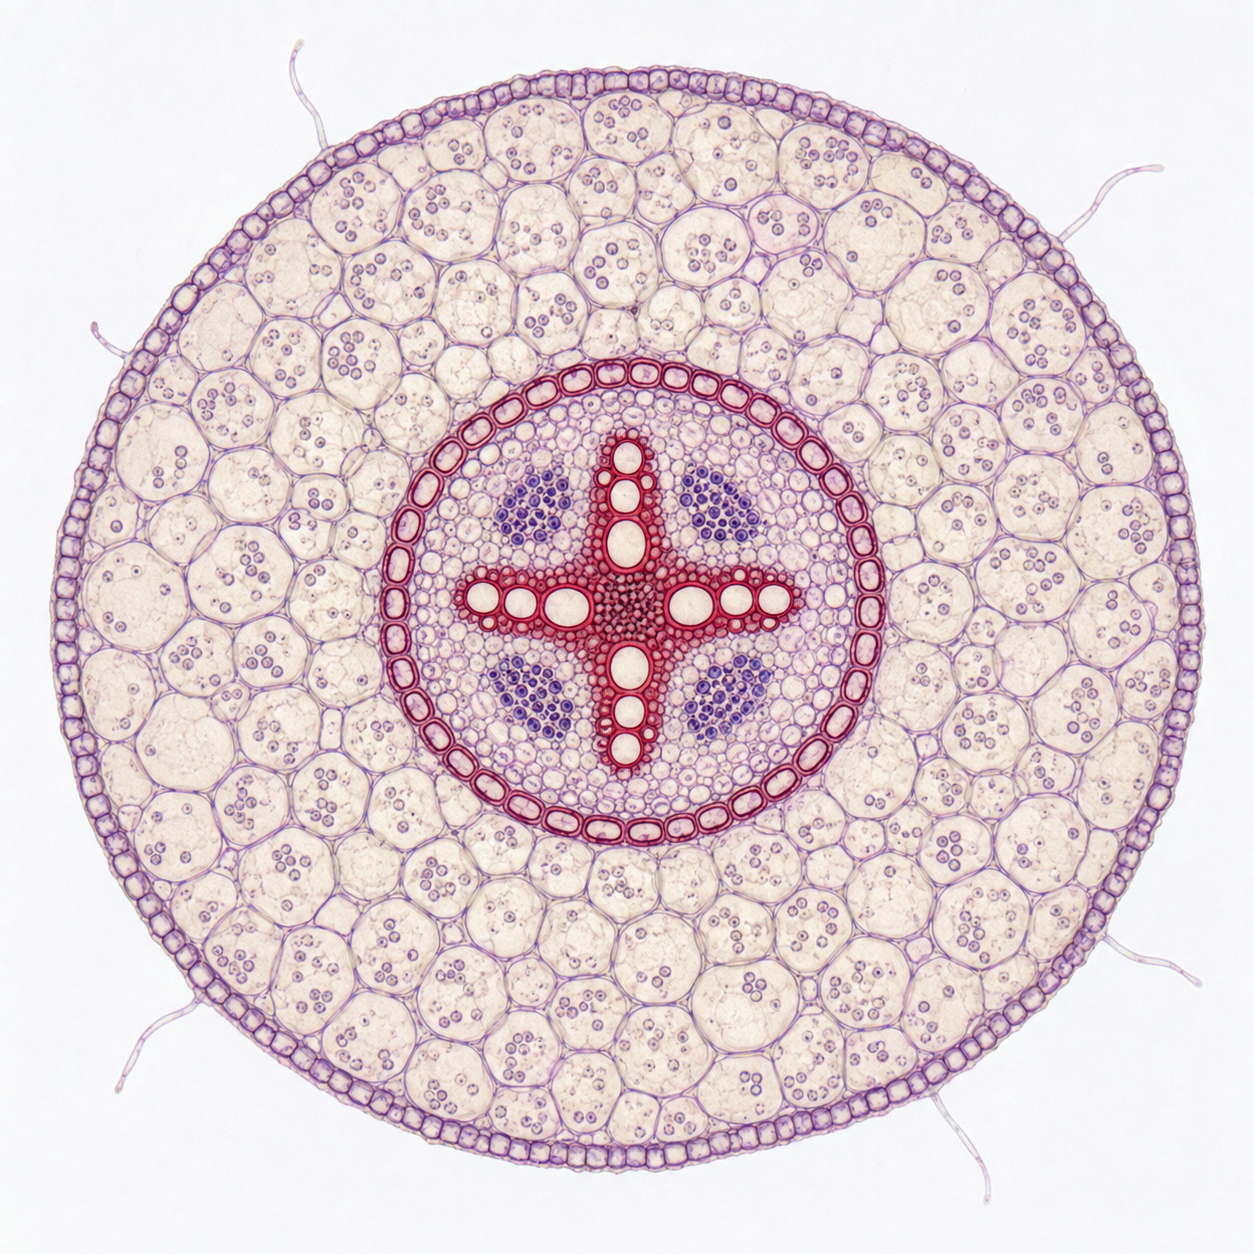
\includegraphics[width=0.46\linewidth]{images/book3/ai/fig-root-cross.png}};
  \begin{scope}[x={(img.south east)}, y={(img.north west)},
      every node/.style={font=\small}]
    \draw[omDef, thick] (0.50,0.52) -- (0.50,1.06) node[above] {نجمة الخشب المركزية};
    \draw[omDef, thick] (0.58,0.45) -- (1.03,0.38) node[right] {لحاء بين الأذرع};
    \draw[omDef, thick] (0.695,0.50) -- (1.03,0.58) node[right] {بشرة داخلية};
    \draw[omDef, thick] (0.30,0.50) -- (-0.03,0.50) node[left] {قشرة};
    \draw[omDef, thick] (0.06,0.62) -- (-0.03,0.74) node[left] {بشرة وأشعار جذرية};
  \end{scope}
\end{tikzpicture}

{\small مقطع عرضي في \omterm{def:b1:flowering-plant-organization:organs}{جذر} فتي ثنائي الفلقة. أسطوانة وعائية مركزية
واحدة: نجمة من \omterm{def:b1:flowering-plant-organization:tissues}{الخشب} \omterm{def:b1:flowering-plant-organization:tissues}{واللحاء} في زواياها، تحدها \omterm{prop:b1:flowering-plant-organization:stemroot}{البشرة الداخلية}؛
وحولها قشرة عريضة؛ وخارجها البشرة الحاملة للأشعار الجذرية.}
\end{omfigure}

\begin{proposition}[الساق والجذر يختلفان في موضع الأنسجة الوعائية]\label{prop:b1:flowering-plant-organization:stemroot}
في الساق الفتي تكوّن الأنسجة الوعائية حزمًا مرتبة في حلقة (ثنائيات
الفلقة) أو مبعثرة في \omterm{def:b1:flowering-plant-organization:tissues}{النسيج الأساسي} (أحاديات الفلقة)، وفي كل حزمة
\omterm{def:b1:flowering-plant-organization:tissues}{خشب} نحو المركز \omterm{def:b1:flowering-plant-organization:tissues}{ولحاء} نحو الخارج؛ ولا \omterm{prop:b1:flowering-plant-organization:stemroot}{بشرة داخلية} هناك، \omterm{def:b1:flowering-plant-organization:tissues}{والنسيج
الأساسي} مقسوم إلى لب مركزي وقشرة خارجية. أما في \omterm{def:b1:flowering-plant-organization:organs}{الجذر} الفتي فأسطوانة
مركزية واحدة: \omterm{def:b1:flowering-plant-organization:tissues}{الخشب} يكوّن نجمة (ذراعان إلى خمسة عند ثنائيات الفلقة،
وكثيرة عند أحادياتها)، \omterm{def:b1:flowering-plant-organization:tissues}{واللحاء} يقع بين الأذرع، وتحد الأسطوانة
\emph{البشرة الداخلية}\index{بشرة داخلية}، وهي حلقة من الخلايا تحمل
جدرها الشعاعية شريطًا كاتمًا للماء (\cref{ch:b1:plant-water-minerals}).
والموضع يوافق الوظيفة: فالساق يقاوم الانحناء، وحلقة من الحزم قرب
سطحه أشد صلابة لكتلتها؛ \omterm{def:b1:flowering-plant-organization:organs}{والجذر} يقاوم الشد، والأسطوانة المركزية هي
ترتيب الكبل.
\end{proposition}

\begin{method}[التعرف على مقطع نباتي]\label{met:b1:flowering-plant-organization:section}
\begin{enumerate}
  \item أسطوانة وعائية مركزية واحدة ذات \omterm{prop:b1:flowering-plant-organization:stemroot}{بشرة داخلية}: \omterm{def:b1:flowering-plant-organization:organs}{جذر}. وحزم في
        حلقة أو مبعثرة، مع لب: ساق. \omterm{def:b1:mammal-organization:organ}{وعضو} مسطح بشرتان له وطبقة
        إسفنجية: \omterm{def:b1:flowering-plant-organization:organs}{ورقة}.
  \item \omterm{def:b1:flowering-plant-organization:organs}{جذر} بأذرع \omterm{def:b1:flowering-plant-organization:tissues}{خشب} قليلة (2--5): ثنائي الفلقة؛ وبأذرع كثيرة حول
        لب: أحادي الفلقة. وساق بحزم في حلقة واحدة: ثنائي الفلقة؛
        وبحزم مبعثرة: أحادي الفلقة.
  \item يُعرف \omterm{def:b1:flowering-plant-organization:tissues}{الخشب} بخلاياه الكبيرة السميكة الجدر الفارغة (حمراء
        بالأصبغة المعتادة)؛ ويُعرف \omterm{def:b1:flowering-plant-organization:tissues}{اللحاء} بخلاياه الحية الصغيرة ذات
        \omterm{def:b1:flowering-plant-organization:tissues}{الأنابيب الغربالية} والخلايا المرافقة (خضراء أو زرقاء).
  \item في مقطع الساق يشير \omterm{def:b1:flowering-plant-organization:tissues}{الخشب} إلى الداخل \omterm{def:b1:flowering-plant-organization:tissues}{واللحاء} إلى الخارج. وفي
        \omterm{def:b1:flowering-plant-organization:organs}{الجذر} يتناوب \omterm{def:b1:flowering-plant-organization:tissues}{الخشب} \omterm{def:b1:flowering-plant-organization:tissues}{واللحاء} على نصف القطر نفسه.
\end{enumerate}
\end{method}

\begin{omfigure}
\begin{tikzpicture}
  \node[anchor=south west, inner sep=0] (img) at (0,0)
    {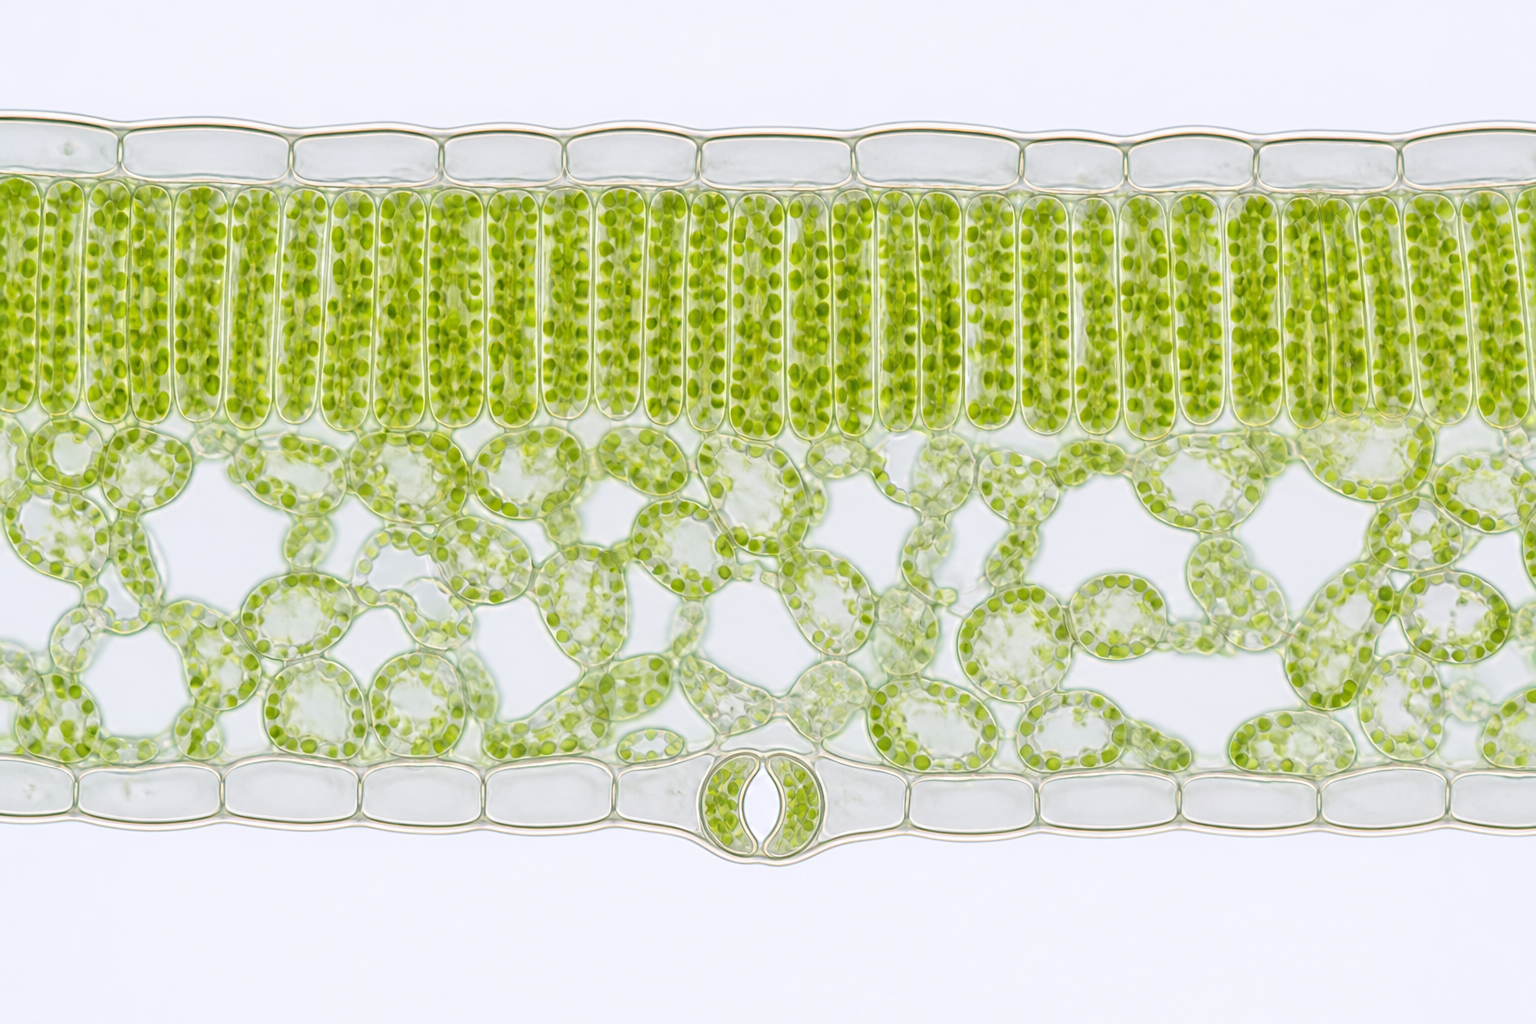
\includegraphics[width=0.48\linewidth]{images/book2/ai/fig-leaf-cross-section.png}};
  \begin{scope}[x={(img.south east)}, y={(img.north west)},
      every node/.style={font=\small}]
    \draw[omDef, thick] (0.50,0.94) -- (0.50,1.08) node[above] {بشرة عليا، أديمة};
    \draw[omDef, thick] (0.30,0.70) -- (-0.03,0.80) node[left] {برنشيم عمادي};
    \draw[omDef, thick] (0.30,0.35) -- (-0.03,0.30) node[left] {برنشيم إسفنجي};
    \draw[omDef, thick] (0.70,0.50) -- (1.03,0.60) node[right] {عرق};
    \draw[omDef, thick] (0.60,0.10) -- (1.03,0.10) node[right] {ثغر};
  \end{scope}
\end{tikzpicture}

{\small مقطع عرضي في \omterm{def:b1:flowering-plant-organization:organs}{ورقة}. بين البشرتين، تواجه الخلايا العمادية
الأسطوانية المكتظة بالبلاستيدات الخضراء الضوءَ، وتترك الخلايا
الإسفنجية المفككة تحتها حيزات هوائية تنفتح عبر الثغور. والعروق تحمل
الماء داخلًا والسكر خارجًا.}
\end{omfigure}

\begin{example}[أين تجري التبادلات]\label{ex:b1:flowering-plant-organization:where}
يدخل ثاني أكسيد الكربون الورقةَ عبر ثغورها، ويعبر حيزات الطبقة
الإسفنجية الهوائية، ويذوب في الجدر المبتلة للخلايا العمادية؛ ويصل
الماء في \omterm{def:b1:flowering-plant-organization:tissues}{خشب} العروق ويخرج بخارًا عبر الثغور نفسها. ويدخل الماء
والشوارد الجذرَ عبر الأشعار الجذرية ويعبران القشرة إلى \omterm{def:b1:flowering-plant-organization:tissues}{الخشب} في
المركز. وكلا العضوين يضع سطح تبادله في الخارج ونسيجه الناقل في
الوسط.
\end{example}

\section{الحياة الثابتة: السطوح}

\begin{definition}[دليل مساحة الأوراق]\label{def:b1:flowering-plant-organization:lai}
\emph{دليل مساحة الأوراق}\index{دليل مساحة الأوراق} $L$ لغطاء نباتي
هو مجموع مساحة \omterm{def:b1:flowering-plant-organization:organs}{الأوراق} من وجه واحد لواحدة مساحة الأرض. ففي مرج في
يونيو يكون $L \approx 3$، وفي غابة نفضية \qtyrange{4}{6}{}، وفي غابة
مطيرة مدارية حتى \qty{8}{}: أي عدة طبقات من الورق مكدسة فوق كل متر
مربع من التربة.
\end{definition}

\begin{proposition}[اعتراض الضوء عند مظلة ورقية]\label{prop:b1:flowering-plant-organization:beer}
الكسر من الضوء الساقط الذي يبلغ الأرض تحت مظلة ورقية دليل مساحة
أوراقها $L$ يتناقص تناقصًا أسيًا،
\[
\frac{I(L)}{I_0} = e^{-kL},
\]
بمعامل خمود $k$ بين $0.3$ (\omterm{def:b1:flowering-plant-organization:organs}{أوراق} منتصبة) و$0.8$ (\omterm{def:b1:flowering-plant-organization:organs}{أوراق} أفقية)،
ونموذجيًا $0.5$. فمظلة عند $L = 5$ مع $k = 0.5$ تعترض
$1 - e^{-2.5} = \qty{92}{\%}$ من الضوء.
\end{proposition}
\begin{proof}
عند الهبوط عبر المظلة، تعترض كل طبقة رقيقة مساحتها الورقية $\dd L$
كسرًا قدره $k\,\dd L$ من الضوء البالغ إليها، حيث $k$ هو كسر المساحة
الأفقية التي تظللها واحدة المساحة الورقية (وهو يتوقف على توجه
\omterm{def:b1:flowering-plant-organization:organs}{الأوراق}). ومن ثم $\dd I = -kI\,\dd L$، وحله هو الأسي.
\end{proof}

\begin{omfigure}
\begin{tikzpicture}
\begin{axis}[
  width=0.86\linewidth, height=6.2cm,
  axis x line=bottom, axis y line=left,
  xmin=0, xmax=9, ymin=0, ymax=1.1,
  xlabel={دليل مساحة الأوراق $L$}, ylabel={كسر الضوء البالغ إلى الأرض},
  xlabel style={font=\small, at={(axis description cs:0.5,-0.12)}, anchor=north},
  ylabel style={font=\small},
  tick label style={font=\small}, xtick={0,2,4,6,8}, ytick={0,0.2,0.4,0.6,0.8,1.0},
  legend style={font=\small, at={(0.97,0.95)}, anchor=north east, draw=none},
  clip=false,
]
\addplot[very thick, omDef, domain=0:9, samples=60] {exp(-0.3*x)};
\addlegendentry{$k = 0.3$ (أوراق منتصبة، نجيليات)}
\addplot[very thick, omThm, domain=0:9, samples=60] {exp(-0.5*x)};
\addlegendentry{$k = 0.5$ (عريض الأوراق النموذجي)}
\addplot[very thick, omProp, domain=0:9, samples=60] {exp(-0.8*x)};
\addlegendentry{$k = 0.8$ (أوراق أفقية)}
\draw[dashed, gray] (axis cs:5,0) -- (axis cs:5,0.082);
\node[font=\scriptsize, anchor=west] at (axis cs:5.3,0.36) {بلوطة، $L=5$: يبقى \qty{8}{\%}};
\end{axis}
\end{tikzpicture}

{\small الضوء تحت مظلة ورقية بدلالة \omterm{def:b1:flowering-plant-organization:lai}{دليل مساحة الأوراق}، من أجل ثلاثة
توجهات \omterm{def:b1:flowering-plant-organization:organs}{للأوراق}. وفوق $L \approx 6$ لا تكسب طبقة \omterm{def:b1:flowering-plant-organization:organs}{أوراق} إضافية شيئًا
يذكر، ولهذا تقف المظلات عندها.}
\end{omfigure}

\begin{proposition}[سطح الجذور يفوق سطح الأوراق]\label{prop:b1:flowering-plant-organization:rootsurface}
نبتة شيلم واحدة نُمّيت أربعة أشهر في صندوق فيه \qty{0.05}{m^3} من
التربة أنتجت \qty{620}{km} من \omterm{def:b1:flowering-plant-organization:organs}{الجذور}، سطحها \qty{240}{m^2}، و
$\num{1.4e10}$ \omterm{def:b1:flowering-plant-organization:organs}{شعرة جذرية} سطحها \qty{400}{m^2} أخرى: أي سطح يناهز
مئة ضعف سطح أوراقها، منشور في التربة بكثافة عشرة كيلومترات من \omterm{def:b1:flowering-plant-organization:organs}{الجذر}
لكل لتر. والأشعار الجذرية، وكل منها امتداد أنبوبي لخلية بشرة واحدة
عرضه \qtyrange{5}{20}{\micro m} وطوله حتى مليمتر، هي موضع معظم
الامتصاص؛ وهي تعيش أيامًا معدودة وتُستبدل كلما تقدمت القمة.
\end{proposition}
\begin{proof}[شواهد]
غسل ديتمر (1937) المجموع الجذري كله لنبتة شيلم واحدة من صندوقها، ثم
عدّ وقاس عينات من كل رتبة جذرية ومن الأشعار الجذرية تحت المجهر، ثم
عمّم: \qty{13.8}{} مليون \omterm{def:b1:flowering-plant-organization:organs}{جذر} مجموعها \qty{623}{km}، و\qty{14}{}
مليار شعرة مجموعها \qty{10620}{km}. وماء التربة وأملاحها تنتقل ببطء
شديد حتى إن على \omterm{def:b1:flowering-plant-organization:organs}{الجذر} أن يكون على بعد مليمتر منها ليأخذها؛ والطول
الهائل هو ما يضع جذرًا في متناول كل قطرة.
\end{proof}

\begin{omfigure}
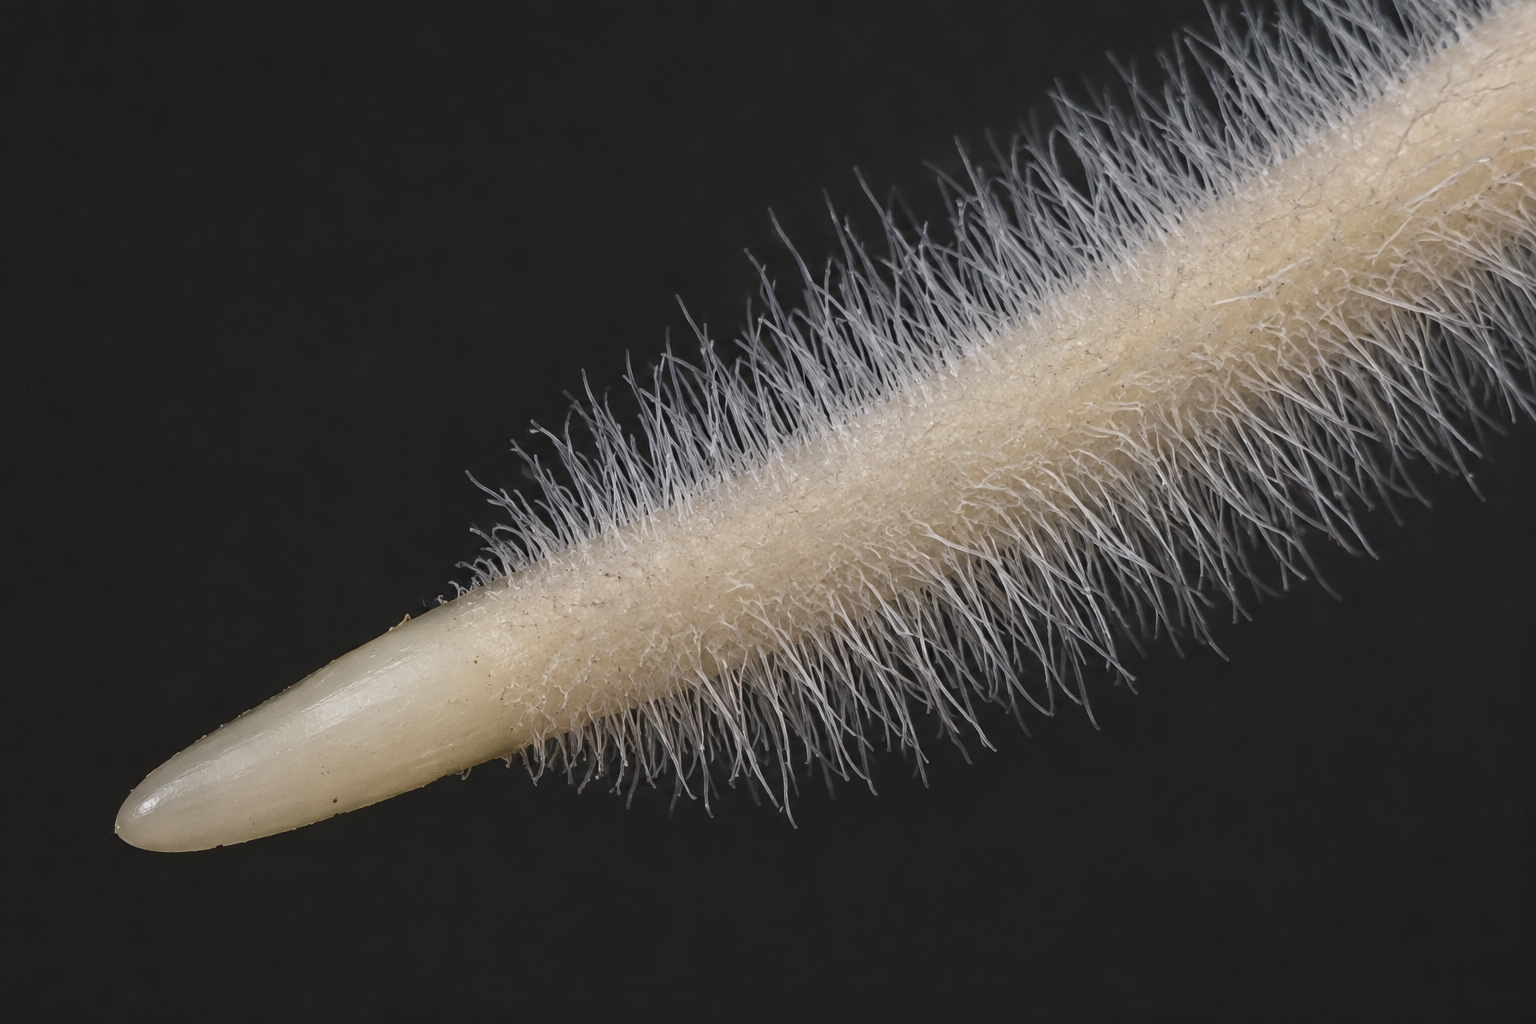
\includegraphics[width=0.58\linewidth]{images/book3/ai/b3-03-root-hairs.png}

{\small أشعار جذرية على بادرة فجل، على بعد بضعة مليمترات خلف القمة
العارية. كل شعرة خلية بشرة واحدة نمت إلى التربة؛ وهي مجتمعة تضاعف
السطح الماص مرات كثيرة.}
\end{omfigure}

\begin{example}[سطحا البلوطة]\label{ex:b1:flowering-plant-organization:oaksurfaces}
بلوطة يظلل تاجها \qty{100}{m^2} عند $L = 5$ تحمل \qty{500}{m^2} من
الورق. أما جذورها الدقيقة، عند بضعة كيلومترات في المتر المكعب عبر
\qty{100}{m^3} من التربة، فتقدم عدة مئات من الأمتار المربعة، وأشعارها
الجذرية ألفًا أخرى: فالسطح الماص تحت الأرض عدة أمثال السطح الضوئي
فوقها، على المتر المربع نفسه من الأرض.
\end{example}

\section{النمو والشكل}

\begin{definition}[النسج الإنشائية، والنمو الأولي والثانوي]\label{def:b1:flowering-plant-organization:meristem}
\emph{النسيج الإنشائي}\index{النسيج الإنشائي} نسيج من خلايا صغيرة غير
متمايزة تظل تنقسم. و\emph{النسج الإنشائية القمية}\index{النسيج الإنشائي القمي} في قمم كل مجموع هوائي وكل \omterm{def:b1:flowering-plant-organization:organs}{جذر} تنتج \emph{النمو
الأولي}\index{النمو الأولي}: الاستطالة، والأنسجة الأولية السابقة.
و\emph{النسج الإنشائية الجانبية}\index{النسيج الإنشائي الجانبي} ---
الكامبيوم الوعائي بين \omterm{def:b1:flowering-plant-organization:tissues}{الخشب} \omterm{def:b1:flowering-plant-organization:tissues}{واللحاء}، وكامبيوم الفلين تحت البشرة ---
تنتج \emph{النمو الثانوي}\index{النمو الثانوي}: التثخن، بإضافة \omterm{def:b1:flowering-plant-organization:tissues}{الخشب}
(\omterm{def:b1:flowering-plant-organization:tissues}{الخشب} الثانوي) إلى الداخل والقلف إلى الخارج، في سيقان الأشجار
والجنبات وجذورها. أما آليات نشاط النسج الإنشائية فتنتمي إلى كتاب
السنة الثانية.
\end{definition}

\begin{omfigure}
\begin{tikzpicture}[font=\small, >=Stealth, line cap=round]
  % root outline (vertical, tip at bottom)
  \draw[thick, omDef!60!black, fill=omDef!8] (-0.7,5.2) -- (-0.7,1.3) .. controls (-0.7,0.4) and (-0.3,0) .. (0,-0.2) .. controls (0.3,0) and (0.7,0.4) .. (0.7,1.3) -- (0.7,5.2);
  % root cap
  \draw[thick, omDef!60!black, fill=omDef!25] (-0.72,0.9) .. controls (-0.75,0.2) and (-0.3,-0.35) .. (0,-0.45) .. controls (0.3,-0.35) and (0.75,0.2) .. (0.72,0.9) .. controls (0.5,0.55) and (0.2,0.4) .. (0,0.45) .. controls (-0.2,0.4) and (-0.5,0.55) .. (-0.72,0.9);
  % meristem
  \fill[omThm!45] (0,0.95) ellipse (0.45 and 0.35);
  % vascular strand
  \draw[thick, omDef!60!black, fill=omDef!30] (-0.15,5.2) -- (-0.15,1.9) .. controls (-0.1,1.5) .. (0,1.35) .. controls (0.1,1.5) .. (0.15,1.9) -- (0.15,5.2);
  % root hairs
  \foreach \y in {3.4,3.7,4.0,4.3,4.6,4.9} { \draw[omDef!60!black] (-0.7,\y) -- (-1.5,\y+0.15); \draw[omDef!60!black] (0.7,\y) -- (1.5,\y+0.15); }
  % zone brackets
  \draw[thick, gray] (2.0,-0.45) -- (2.2,-0.45) -- (2.2,0.6) -- (2.0,0.6); \node[right, align=left, font=\footnotesize] at (2.3,0.1) {القلنسوة الجذرية: تحمي القمة،\\ وتحس الجاذبية};
  \draw[thick, gray] (2.0,0.6) -- (2.2,0.6) -- (2.2,1.4) -- (2.0,1.4); \node[right, align=left, font=\footnotesize] at (2.3,1.0) {منطقة الانقسام:\\ النسيج الإنشائي القمي (أحمر)};
  \draw[thick, gray] (2.0,1.4) -- (2.2,1.4) -- (2.2,3.1) -- (2.0,3.1); \node[right, align=left, font=\footnotesize] at (2.3,2.25) {منطقة الاستطالة: تطول\\ الخلايا عشرة أضعاف، فتدفع\\ القمة عبر التربة};
  \draw[thick, gray] (2.0,3.1) -- (2.2,3.1) -- (2.2,5.2) -- (2.0,5.2); \node[right, align=left, font=\footnotesize] at (2.3,4.15) {منطقة التمايز:\\ أشعار جذرية، وخشب ولحاء\\ ناضجان};
  \node[left, font=\footnotesize, align=right] at (-1.6,4.4) {أشعار جذرية};
  \node[left, font=\footnotesize, align=right] at (-0.85,2.4) {الأسطوانة\\ الوعائية\\ في التكوّن};
\end{tikzpicture}

{\small مقطع طولي في قمة \omterm{def:b1:flowering-plant-organization:organs}{جذر}. خلف القلنسوة الواقية ينقسم \omterm{def:b1:flowering-plant-organization:meristem}{النسيج
الإنشائي القمي}؛ ثم تستطيل نواتجه، ثم تتمايز إلى أنسجة \omterm{def:b1:flowering-plant-organization:organs}{الجذر} الناضج
وتنبت \omterm{def:b1:flowering-plant-organization:organs}{أشعارًا جذرية}. والتتابع كله يشغل بضعة مليمترات ويتقدم كلما نما
\omterm{def:b1:flowering-plant-organization:organs}{الجذر}.}
\end{omfigure}

\begin{proposition}[الشكل يتبع الموقع]\label{prop:b1:flowering-plant-organization:plasticity}
لأن نموه \omterm{prop:b1:flowering-plant-organization:modular}{وحدوي} \omterm{prop:b1:flowering-plant-organization:modular}{غير محدود}، يشكّل النبات جسمه على موقعه
(\emph{المرونة الظاهرية}\index{المرونة الظاهرية}): فالشجرة النامية
في العراء تتفرع منخفضة عريضة، والنوع نفسه في غابة ينمو جذعًا عاريًا
طويلًا؛ والنبات في تربة جافة يخصص لجذوره حصة أكبر من نموه، وفي الظل
يخصص لأوراقه. وأنواع الموائل الجافة (\emph{النباتات
الجفافية}\index{نبات جفافي}) تحمل أديمات سميكة، وثغورًا غائرة في حفر
أو محمية بأشعار، وأوراقًا صغيرة أو عصيرية، وجذورًا عميقة؛ وأنواع
الموائل الرطبة (\emph{النباتات المائية}\index{نبات مائي}) تحمل أديمات
رقيقة، وثغورًا على الوجه العلوي \omterm{def:b1:flowering-plant-organization:organs}{لأوراق} طافية، ونسيجًا مملوءًا هواءً
(\emph{النسيج الهوائي}\index{النسيج الهوائي}) يحمل الأكسجين إلى
\omterm{def:b1:flowering-plant-organization:organs}{الجذور} في الوحل عديم الأكسجين.
\end{proposition}

\begin{example}[ثديي ونبات، جنبًا إلى جنب]\label{ex:b1:flowering-plant-organization:comparison}
التغذية: الثديي يأكل مادة عضوية؛ والنبات يصنعها من ثاني أكسيد
الكربون والماء والضوء. سطوح التبادل: داخلية ثابتة القياس مروية
بالدم؛ وخارجية نامية تهويها الريح والتربة. \omterm{def:b1:organism-environment:milieu}{الوسط الداخلي}: سائل
منظَّم ثابت الحرارة والتركيب؛ ولا شيء --- فالخلايا تنظم محتوياتها
وحرارة النبات هي حرارة الهواء. النمو: إلى شكل بالغ محدد؛ ومفتوح
\omterm{prop:b1:flowering-plant-organization:modular}{وحدوي} مدى الحياة. الحركة: الحيوان يذهب إلى غذائه؛ والنبات ينمو نحو
الضوء والماء. التنسيق: أعصاب وهرمونات في ثوان إلى ساعات؛ وهرمونات
وحدها في ساعات إلى أيام. وكل عمود طريقة متسقة في أن تكون نظامًا
مفتوحًا.
\end{example}

\section{تمارين}

\begin{exercise}[$\star$]\label{exo:b1:flowering-plant-organization:1}
اذكر \omterm{def:b1:mammal-organization:organ}{الأعضاء} الخضرية الثلاثة للنبات الزهري والوظيفة الرئيسة لكل
منها.
\end{exercise}

\begin{exercise}[$\star$]\label{exo:b1:flowering-plant-organization:2}
عرّف وحدة المجموع الهوائي وفسّر ما معنى «\omterm{prop:b1:flowering-plant-organization:modular}{النمو غير المحدود}».
\end{exercise}

\begin{exercise}[$\star$]\label{exo:b1:flowering-plant-organization:3}
من أجل كل نسيج --- البشرة، \omterm{def:b1:flowering-plant-organization:tissues}{والبرنشيم}، \omterm{def:b1:flowering-plant-organization:tissues}{والكولنشيم}، \omterm{def:b1:flowering-plant-organization:tissues}{والسكلرنشيم}،
\omterm{def:b1:flowering-plant-organization:tissues}{والخشب}، \omterm{def:b1:flowering-plant-organization:tissues}{واللحاء} --- قل هل خلاياه حية عند النضج وما الذي يفعله.
\end{exercise}

\begin{exercise}[$\star$]\label{exo:b1:flowering-plant-organization:4}
من شكل اعتراض الضوء، ما الكسر من الضوء الذي يبلغ الأرض تحت مرج عند
$L = 3$ مع $k = 0.3$، وتحت غابة عريضة \omterm{def:b1:flowering-plant-organization:organs}{الأوراق} عند $L = 6$ مع
$k = 0.5$؟
\end{exercise}

\begin{exercise}[$\star\star$]\label{exo:b1:flowering-plant-organization:5}
يبين مقطع نجمة \omterm{def:b1:flowering-plant-organization:tissues}{خشب} مركزية بأربعة أذرع، \omterm{def:b1:flowering-plant-organization:tissues}{ولحاء} بين الأذرع، وحلقة من
الخلايا ذات جدر شعاعية مثخنة حولها، ومنطقة عريضة من الخلايا
المستديرة خارجها. عيّن \omterm{def:b1:mammal-organization:organ}{العضو} والمجموعة، مع ذكر الخاصيتين اللتين
تحسمان كلًا منهما.
\end{exercise}

\begin{exercise}[$\star\star$]\label{exo:b1:flowering-plant-organization:6}
فسّر، مستعينًا بميكانيك العارضة والكبل، لماذا يقع \omterm{def:b1:flowering-plant-organization:tissues}{النسيج الوعائي} في
حلقة محيطية في الساق وفي أسطوانة مركزية في \omterm{def:b1:flowering-plant-organization:organs}{الجذر}.
\end{exercise}

\begin{exercise}[$\star\star$]\label{exo:b1:flowering-plant-organization:7}
محصول عنده $L = 4$ و$k = 0.6$. ما الكسر من الضوء الذي يعترضه؟ وبكم
يرتفع الاعتراض لو صار $L$ يساوي 6؟ علّق على مردود \omterm{def:b1:flowering-plant-organization:organs}{الأوراق} الزائدة.
\end{exercise}

\begin{exercise}[$\star\star$]\label{exo:b1:flowering-plant-organization:8}
نبتة الشيلم عند ديتمر كان لها \qty{623}{km} من \omterm{def:b1:flowering-plant-organization:organs}{الجذور}
و\qty{240}{m^2} من السطح الجذري. احسب القطر الوسطي \omterm{def:b1:flowering-plant-organization:organs}{للجذر}. وإذا كان
مجموع أوراقها \qty{5}{m^2}، فما نسبة سطح \omterm{def:b1:flowering-plant-organization:organs}{الجذور} مع الأشعار إلى سطح
\omterm{def:b1:flowering-plant-organization:organs}{الأوراق}؟
\end{exercise}

\begin{exercise}[$\star\star$]\label{exo:b1:flowering-plant-organization:9}
أشعار جذرية عرضها $\qty{10}{\micro m}$ وطولها $\qty{0.8}{mm}$،
بمعدل \qty{250}{} لكل مليمتر من \omterm{def:b1:flowering-plant-organization:organs}{الجذر}. بأي عامل تضاعف سطح \omterm{def:b1:flowering-plant-organization:organs}{جذر} قطره
$\qty{0.4}{mm}$؟
\end{exercise}

\begin{exercise}[$\star\star\star$]\label{exo:b1:flowering-plant-organization:10}
شجرة في غابة لها جذع عار طوله \qty{20}{m} وتاج صغير؛ والنوع نفسه في
حقل عريض متفرع من \qty{2}{m}. فسّر الشكلين انطلاقًا من \omterm{prop:b1:flowering-plant-organization:modular}{النمو
الوحدوي} ومن مصير البراعم الإبطية في الظل وفي الضوء، وقل ماذا تكلف
هذه المرونة وماذا تكسب.
\end{exercise}

\begin{exercise}[$\star\star\star$]\label{exo:b1:flowering-plant-organization:11}
\omterm{prop:b1:flowering-plant-organization:plasticity}{نبات جفافي} ثغوره غائرة في حفر مبطنة بأشعار. فسّر ماذا يفعل هذا
بتدرج بخار الماء بين حيزات \omterm{def:b1:flowering-plant-organization:organs}{الورقة} الهوائية والريح، وماذا يكلف في
أخذ ثاني أكسيد الكربون. ولماذا كانت هذه مقايضة رابحة في صحراء
وخاسرة في غابة مطيرة؟
\end{exercise}

\begin{exercise}[$\star\star\star$]\label{exo:b1:flowering-plant-organization:12}
«لا \omterm{def:b1:organism-environment:milieu}{وسط داخلي} للنبات.» ناقش في فقرة: ما الذي يفتقر إليه النبات مما
يملكه الثديي، وما الذي تواجهه خلاياه نتيجة لذلك، وما الذي يفعله بدلًا
من ذلك --- السطوح، والنمو، والتنظيم الذي يقوم به فعلًا.
\end{exercise}

\section{مسألة: سطوح بلوطة}

\begin{problem}[{مسألة نهاية الأسبوع --- أوراق بلوطة معدودة بالمساحة،
وثغورها بالمليارات، وكربونها وماؤها بالكيلوغرام، وجذورها
بالكيلومتر، وصولًا إلى سطح التبادل الذي تنشره فوق كل متر مربع من
أرضها}]
\label{pb:b1:flowering-plant-organization:1}
بلوطة يظلل تاجها \qty{100}{m^2} من الأرض بدليل مساحة \omterm{def:b1:flowering-plant-organization:organs}{أوراق} $L = 5$
ومعامل خمود $k = 0.5$. وأوجه أوراقها السفلى تحمل \qty{150}{} ثغرًا
في المليمتر المربع؛ والفتحة الثغرية المفتوحة \qty{10}{\micro m} في
\qty{5}{\micro m}. وبالمتوسط على المظلة كلها وعلى نهار طوله
\qty{12}{h}، يأخذ كل متر مربع من الورق \qty{4}{\micro mol} من
$\mathrm{CO_2}$ ويفقد \qty{1}{mmol} من بخار الماء في الثانية.
\omterm{def:b1:flowering-plant-organization:organs}{والجذور} الدقيقة (قطرها \qty{0.5}{mm}) تمتد \qty{5}{km} في المتر
المكعب عبر \qty{1}{m} من عمق التربة تحت التاج؛ والأشعار الجذرية
(\qty{10}{\micro m} في \qty{0.5}{mm}) تنبت بمعدل \qty{200}{} لكل
مليمتر من \omterm{def:b1:flowering-plant-organization:organs}{الجذر} الدقيق. والكتل المولية: $\mathrm{CO_2}$
\qty{44}{g/mol}، والكربون \qty{12}{g/mol}، و$\mathrm{H_2O}$
\qty{18}{g/mol}.

\medskip
\noindent\textbf{الجزء الأول --- \omterm{def:b1:flowering-plant-organization:organs}{الأوراق} والضوء.}
\begin{enumerate}
  \item احسب مجموع مساحة \omterm{def:b1:flowering-plant-organization:organs}{أوراق} التاج من وجه واحد.
  \item احسب الكسر من الضوء البالغ إلى الأرض والكسر المعترَض.
  \item احسب الكسر المعترَض لو لم يكن للبلوطة إلا $L = 2$، ولو كان
        لها $L = 8$.
  \item فسّر من هذه الأعداد لماذا تقف البلوطة عند $L \approx 5$.
  \item \omterm{def:b1:flowering-plant-organization:organs}{الورقة} الوسطية \qty{50}{cm^2}. فكم \omterm{def:b1:flowering-plant-organization:organs}{ورقة} يحمل التاج؟
\end{enumerate}

\medskip
\noindent\textbf{الجزء الثاني --- الثغور والكربون.}
\begin{enumerate}[resume]
  \item احسب عدد الثغور على التاج.
  \item احسب مساحة فتحة مفتوحة واحدة والكسر من سطح \omterm{def:b1:flowering-plant-organization:organs}{الورقة} السفلي
        الذي تمثله الفتحات المفتوحة.
  \item احسب أخذ التاج من $\mathrm{CO_2}$ بالمول في الثانية
        وبالغرام في الثانية.
  \item احسب $\mathrm{CO_2}$ المأخوذ في نهار واحد طوله \qty{12}{h}،
        بالكيلوغرام، والكربون الذي يحويه.
  \item على موسم نمو طوله \qty{150}{} يومًا، كم كربونًا يثبت التاج؟
        وإذا تنفس النبات نصفه، فأي كتلة من \omterm{def:b1:flowering-plant-organization:tissues}{الخشب} (\qty{50}{\%}
        كربون) يستطيع أن يضيف؟
\end{enumerate}

\medskip
\noindent\textbf{الجزء الثالث --- الماء.}
\begin{enumerate}[resume]
  \item احسب الماء الذي يفقده التاج بالمول وبالغرام في الثانية.
  \item احسب الفقد المائي اليومي باللتر.
  \item احسب نسبة جزيئات الماء المفقودة إلى جزيئات $\mathrm{CO_2}$
        المكتسبة. ولماذا كانت كبيرة إلى هذا الحد؟
  \item مطر مقداره \qty{2}{mm} يسقط على \qty{100}{m^2}. فكم يومًا من
        النتح يغطي، إذا بلغ كله \omterm{def:b1:flowering-plant-organization:organs}{الجذور}؟
\end{enumerate}

\medskip
\noindent\textbf{الجزء الرابع --- \omterm{def:b1:flowering-plant-organization:organs}{الجذور}.}
\begin{enumerate}[resume]
  \item احسب حجم التربة المستكشَفة والطول الكلي \omterm{def:b1:flowering-plant-organization:organs}{للجذور} الدقيقة.
  \item احسب سطح \omterm{def:b1:flowering-plant-organization:organs}{الجذور} الدقيقة (بوصفها أسطوانات).
  \item احسب عدد الأشعار الجذرية.
  \item احسب سطح الأشعار الجذرية.
  \item احسب مجموع السطح الماص تحت الأرض، ونسبته إلى مساحة \omterm{def:b1:flowering-plant-organization:organs}{الأوراق}
        من وجه واحد.
  \item \omterm{def:b1:flowering-plant-organization:organs}{الجذور} الدقيقة على بعد \qty{1}{mm} من أي كسر من حجم التربة؟
        (اعتبر كل \omterm{def:b1:flowering-plant-organization:organs}{جذر} محورًا لأسطوانة نصف قطرها \qty{1}{mm}.)
  \item قارن مع نبتة الشيلم في هذا الفصل (\qty{620}{km} من \omterm{def:b1:flowering-plant-organization:organs}{الجذور}
        في \qty{0.05}{m^3}): أي النبتتين تستكشف تربتها استكشافًا
        أدق، وبأي عامل؟
  \item اجمع مساحة \omterm{def:b1:flowering-plant-organization:organs}{الأوراق} من الوجهين وسطح \omterm{def:b1:flowering-plant-organization:organs}{الجذور}. واقسم على
        \qty{100}{m^2} من الأرض.
  \item قارن هذا مع نسبة سطوح التبادل المطوية (\qty{130}{m^2}) إلى
        السطح الخارجي (\qty{2}{m^2}) عند الإنسان.
  \item فسّر في جملتين لماذا تستطيع نسبة النبات أن تظل ترتفع طول
        حياته ولا تستطيع نسبة الثديي ذلك.
  \item اذكر النتيجة: \omterm{prop:b1:organism-environment:surfaces}{سطح التبادل} الذي تنشره بلوطة لكل متر مربع من
        أرضها، فوقها وتحتها، بالمتر المربع.
\end{enumerate}
\end{problem}
